% Three-loop selectable controller cascade map.
% Compile: pdflatex algorithm-map.tex && pdf2svg ...
\documentclass[tikz, margin=4mm]{standalone}
\usetikzlibrary{arrows.meta, positioning, calc, fit, backgrounds}

\tikzset{
  loop/.style  = {draw, rectangle, rounded corners=4pt, align=center,
                  fill=blue!6, font=\small, inner sep=6pt,
                  minimum width=8.0cm, minimum height=1.3cm},
  aug/.style   = {draw, rectangle, rounded corners=4pt, align=center,
                  fill=orange!10, font=\small, inner sep=4pt,
                  minimum width=3.5cm},
  sensor/.style = {draw, rectangle, rounded corners=4pt, align=center,
                   fill=gray!10, font=\small, inner sep=4pt},
  arr/.style   = {-{Latex[length=4pt, width=5pt]}, thick},
  lbl/.style   = {font=\small},
  node distance = 0.6cm and 1.2cm
}

\begin{document}
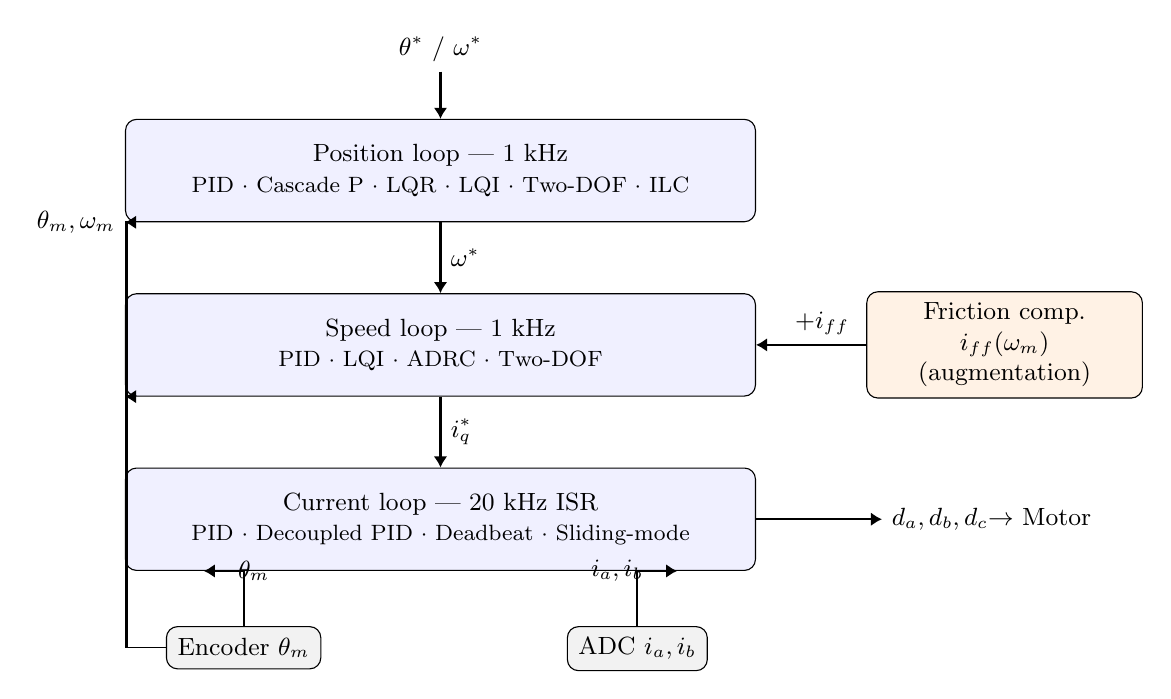
\begin{tikzpicture}

  % ── Three control loops (stacked vertically) ──────────────────────────────
  \node[loop] (PosLoop)
    {Position loop — 1 kHz\\
     \footnotesize PID $\cdot$ Cascade P $\cdot$ LQR $\cdot$ LQI $\cdot$ Two-DOF $\cdot$ ILC};

  \node[loop, below=0.9cm of PosLoop] (SpdLoop)
    {Speed loop — 1 kHz\\
     \footnotesize PID $\cdot$ LQI $\cdot$ ADRC $\cdot$ Two-DOF};

  \node[loop, below=0.9cm of SpdLoop] (CurLoop)
    {Current loop — 20 kHz ISR\\
     \footnotesize PID $\cdot$ Decoupled PID $\cdot$ Deadbeat $\cdot$ Sliding-mode};

  % ── Friction compensation (augmentation, beside speed loop) ───────────────
  \node[aug, right=1.4cm of SpdLoop] (FricComp)
    {Friction comp.\\ $i_{ff}(\omega_m)$\\ (augmentation)};

  % ── Sensors ───────────────────────────────────────────────────────────────
  \node[sensor, below=0.7cm of CurLoop, xshift=-2.5cm] (Enc)
    {Encoder $\theta_m$};
  \node[sensor, below=0.7cm of CurLoop, xshift=2.5cm]  (Adc)
    {ADC $i_a,i_b$};

  % ── Motor output ──────────────────────────────────────────────────────────
  \node[lbl, right=1.6cm of CurLoop] (Motor) {$d_a,d_b,d_c$\\ $\rightarrow$ Motor};

  % ── Reference input ───────────────────────────────────────────────────────
  \node[lbl, above=0.6cm of PosLoop] (Ref) {$\theta^*$ / $\omega^*$};

  % ── Cascade connections ───────────────────────────────────────────────────
  \draw[arr] (Ref.south)     -- node[lbl,right]{} (PosLoop.north);
  \draw[arr] (PosLoop.south) -- node[lbl,right]{$\omega^*$} (SpdLoop.north);
  \draw[arr] (SpdLoop.south) -- node[lbl,right]{$i_q^*$}    (CurLoop.north);
  \draw[arr] (CurLoop.east)  -- (Motor.west);

  % ── Friction augmentation path ────────────────────────────────────────────
  \draw[arr] (FricComp.west) -- node[lbl,above,pos=0.4]{$+i_{ff}$}
             ($(SpdLoop.east)+(0,0)$);

  % ── Sensor feedback ───────────────────────────────────────────────────────
  \draw[arr] (Enc.north) |-
             node[lbl,right,pos=0.7]{$\theta_m$}
             ($(CurLoop.south west)+(1.0,-0.0)$);
  \draw[arr] (Adc.north) |-
             node[lbl,left,pos=0.7]{$i_a,i_b$}
             ($(CurLoop.south east)+(-1.0,0)$);

  % encoder also feeds outer loops
  \coordinate (EncFb) at ($(Enc.west)+(-0.5,0)$);
  \draw (Enc.west) -- (EncFb);
  \draw[arr] (EncFb) |-
             node[lbl,left,pos=0.8]{$\theta_m,\omega_m$}
             (PosLoop.south west);
  \draw[arr] (EncFb) |-
             (SpdLoop.south west);

\end{tikzpicture}
\end{document}
